\chapter{Feature Engineering}
\label{ch:feature}

The windowed dataset from \Cref{ch:processing} consists of \SI{2}{\second} segments of synchronised, filtered IMU and odometry samples. Before any classifier can be trained, each window must be summarised by a fixed-length feature vector that is approximately stationary within the window and informative about the underlying terrain. This chapter describes the feature design, the two speed-regime dataset variants derived from the resulting feature table, and the data-driven feature-selection procedure used to control dimensionality before modelling. All feature logic lives in \texttt{src/features.py} and is invoked from \texttt{06\_features.ipynb} (5-class campus and 3-class farm extraction) and \texttt{06b\_features\_dataset\_B\_3class.ipynb} (read-only re-analysis on the modelling subset). The theoretical motivation, together with the definitions of Hjorth, band-power, spectral and mutual-information quantities, was given in \Cref{sec:bg-features-ml}; this chapter focuses on the concrete implementation choices.

\paragraph{Input channels.}
Five raw IMU channels are used: the three accelerometer axes $(a_x, a_y, a_z)$ and two gyroscope axes $(g_x, g_z)$. The yaw rate $g_y$ is excluded throughout (cf.\ \Cref{sec:bg-proprio,ch:setup}), as it is dominated by intentional steering rather than terrain-induced motion, and including it would let a classifier learn route-specific cues. Two derived \emph{magnitude} channels are also computed per window,
\begin{equation}
    \lVert \mathbf{a}\rVert(n) = \sqrt{a_x^2(n) + a_y^2(n) + a_z^2(n)},
    \qquad
    \lVert \mathbf{g}\rVert(n) = \sqrt{g_x^2(n) + g_z^2(n)},
    \label{eq:magnitudes}
\end{equation}
capturing overall vibration intensity in an orientation-agnostic form. The accelerometer magnitude is computed \emph{after} per-window mean removal on each axis: the mean of $a_y$ contains the $\approx{-1}\,g$ gravity component plus residual DC bias, and subtracting it leaves only dynamic, terrain-driven acceleration. The same DC-removal step is used downstream in the per-axis time-domain features.

\paragraph{Feature groups.}
For each of the seven channels (five raw IMU plus two magnitudes), the same suite of time-domain (\Cref{sec:feat_time}) and frequency-domain (\Cref{sec:feat_freq}) descriptors is computed, complemented by four within-sensor and four cross-sensor correlations and three odometry features summarising the wheel-speed signal within the window. The resulting feature vector contains $189$ entries (186 IMU and odometry features plus three optional speed-normalised energy descriptors, gated by a configuration flag in the extraction notebook), and is reduced substantially by the selection step in \Cref{sec:feat_selection}.

\begin{figure}[H]
    \centering
    \begin{tikzpicture}[
        font=\small,
        box/.style={draw, rounded corners=2pt, align=center,
                    inner sep=3pt, minimum height=3mm, text width=24mm},
        inp/.style={box, fill=gray!15},
        feat/.style={box, fill=blue!8},
        out/.style={box, fill=green!12, font=\footnotesize\bfseries},
        arr/.style={-{Latex[length=1mm]}, semithick}
    ]
    % Input
    \node[inp, text width=42mm] (sig) at (0,0) {Windowed signals (\SI{2}{\second})};

    % Parallel feature-extraction branches
    \node[feat] (tf)  at (-5.2,-1.7)  {Time + frequency\\descriptors};
    \node[feat] (mag) at (-1.75,-1.7) {Magnitudes\\$\lVert\mathbf{a}\rVert,\;\lVert\mathbf{g}\rVert$};
    \node[feat] (xc)  at ( 1.75,-1.7) {Within- \& cross-\\sensor correlations};
    \node[feat] (od)  at ( 5.2,-1.7) {Odometry\\features};

    % Raw feature table (with speed-normalised features folded in)
    \node[box, text width=72mm] (raw) at (0,-3.4)
        {Raw feature table \;($186 + 3$ speed-normalised $\Rightarrow d=189$)};

    % Per-dataset processing (split + log-transform + pruning in one box)
    \node[box, text width=46mm] (pA) at (-4.2,-5.1)
        {Dataset A (all speeds)\\log-transform $\to$ corr.\ pruning};
    \node[box, text width=46mm] (pB) at ( 4.2,-5.1)
        {Dataset B (low, constant speed)\\log-transform $\to$ corr.\ pruning};

    % Final outputs
    \node[out] (fA) at (-4.2,-6.6) {Final table A};
    \node[out] (fB) at ( 4.2,-6.6) {Final table B};

    % Arrows
    \draw[arr] (sig.south) -- (tf.north);
    \draw[arr] (sig.south) -- (mag.north);
    \draw[arr] (sig.south) -- (xc.north);
    \draw[arr] (sig.south) -- (od.north);

    \draw[arr] (tf.south)  -- (raw.north);
    \draw[arr] (mag.south) -- (raw.north);
    \draw[arr] (xc.south)  -- (raw.north);
    \draw[arr] (od.south)  -- (raw.north);

    \draw[arr] (raw.south) -- (pA.north);
    \draw[arr] (raw.south) -- (pB.north);
    \draw[arr] (pA) -- (fA);
    \draw[arr] (pB) -- (fB);

    \end{tikzpicture}
    \caption{Feature-engineering pipeline from windowed signals to the pruned, model-ready feature tables. Mutual information ranking is computed only for EDA; the actual dimensionality reduction is the $|\rho|>0.95$ correlation pruning, with the three speed/odometry columns excluded from aggressive removal.}
    \label{fig:feature_pipeline}
\end{figure}

\section{Time-Domain Features}
\label{sec:feat_time}

Each of the seven channels $x[n]$ defined above is passed through the same time-domain extractor, producing three families of per-channel descriptors and a small set of pairwise correlations computed once per window.

\subsection{Distributional and Shape Statistics}

The first family summarises the marginal distribution of the windowed signal through ten descriptors: mean, standard deviation, minimum, maximum, range, median, interquartile range, mean absolute value, skewness $\gamma_1$ and kurtosis $\gamma_2$. The latter two are computed in their unbiased Fisher--Pearson forms
\begin{equation}
    \gamma_1 = \frac{\sqrt{N(N-1)}}{N-2}\,\frac{m_3}{m_2^{3/2}},
    \qquad
    \gamma_2 = \frac{(N+1)(N-1)}{(N-2)(N-3)}\,\frac{m_4}{m_2^{2}} - \frac{3(N-1)^{2}}{(N-2)(N-3)},
    \label{eq:skew_kurt}
\end{equation}
where $m_k = \tfrac{1}{N}\sum_n (x[n]-\bar x)^{k}$ is the central moment of order $k$ (\texttt{scipy.stats.skew} and \texttt{kurtosis} with \texttt{bias=False}). Both quantities are particularly informative on cobblestone and dirt-track surfaces, whose impulsive vibration produces heavy-tailed (high-kurtosis) per-window distributions distinguishable from smoother, near-Gaussian surfaces.

\subsection{Energy and Crossing-Rate Features}

The second family captures signal energy and zero-crossing behaviour: root-mean-square $\mathrm{RMS}(x) = \sqrt{\frac{1}{N}\sum_{n=0}^{N-1} x^{2}[n]}$, total energy $E(x)=\sum_{n} x^{2}[n]$, and the zero-crossing rate
\begin{equation}
    \mathrm{ZCR}(x) = \frac{1}{N-1}\sum_{n=1}^{N-1} \mathbb{1}\bigl\{x[n]\,x[n-1] < 0\bigr\},
    \label{eq:zcr}
\end{equation}
which counts sign changes between adjacent samples. Acceleration RMS is among the most reliably discriminative single features in the IMU terrain-classification literature~\cite{Brooks2005,Weiss2011}.

\subsection{Hjorth Parameters and Jerk}

The third family captures derivative-based dynamics. Hjorth's activity, mobility and complexity (\Cref{eq:hjorth-activity,eq:hjorth-mobility,eq:hjorth-complexity}) give compact estimates of signal power, mean frequency and bandwidth from discrete differences alone, without an explicit Fourier transform~\cite{Hjorth1970}. Jerk RMS (\Cref{eq:jerk-rms}), the root-mean-square of the first time derivative of acceleration, discriminates between hard, impulsive surfaces (high jerk) and compliant ones (low jerk); applied to $g_x$ and $g_z$, it likewise captures the impulsiveness of pitch and roll responses, which differ markedly between, for example, smooth tarmac and an irregular cobblestone yard. Hjorth complexity and jerk RMS on the gyroscope channels in fact occupy the top tier of the dataset-A mutual-information ranking (\Cref{sec:feat_selection}).

\subsection{Within- and Cross-Sensor Correlations}

In addition to the per-channel features, eight Pearson correlations are computed once per window. Three are \emph{within-sensor} accelerometer pairs (lateral--vertical, lateral--longitudinal, vertical--longitudinal) and one is the within-gyroscope pitch--roll pair. The remaining four are \emph{cross-sensor} accelerometer--gyroscope pairs that encode the joint linear--rotational signature of wheel--terrain interaction:
\begin{equation}
    \rho_{a_y,\,g_x},\quad
    \rho_{a_y,\,g_z},\quad
    \rho_{a_z,\,g_x},\quad
    \rho_{a_x,\,g_z}.
    \label{eq:cross_corrs}
\end{equation}
Each pair has a direct physical reading: $\rho_{a_y,g_x}$ and $\rho_{a_y,g_z}$ couple vertical bounce with pitch and roll (typical of soft or muddy terrain, where the nose dips in or the left--right wheels sink unevenly), while $\rho_{a_z,g_x}$ and $\rho_{a_x,g_z}$ couple longitudinal and lateral acceleration with pitch and roll (bump-cresting and side-sloped surfaces, respectively). These cross-sensor terms cannot be recovered by any per-channel feature and provide complementary, physically interpretable information about wheel--terrain coupling, even though they do not rank in the top tier of the dataset-A mutual-information ranking, where derivative-based descriptors (Hjorth, jerk RMS) and low-band spectral power dominate (\Cref{sec:feat_selection}).

\section{Frequency-Domain Features}
\label{sec:feat_freq}

The same seven channels are transformed into the frequency domain via the discrete Fourier transform (DFT) for the second family of features. Each centred window $\tilde x[n] = x[n] - \bar x$ is converted to a periodogram estimate of the power spectral density (PSD),
\begin{equation}
    S_{xx}(f_k) = \frac{1}{N}\,|\hat{X}(f_k)|^{2},
    \qquad
    \hat{X}(f_k) = \sum_{n=0}^{N-1} \tilde x[n]\,e^{-j 2\pi k n / N},
    \label{eq:psd}
\end{equation}
with $f_k = k\,f_s / N$ for $k = 0, 1, \dots, N/2$. At the chosen window length and sample rate ($W = \SI{2}{\second}$, $f_s = \SI{100}{\hertz}$, $N=200$), the frequency resolution is $\Delta f = f_s/N = \SI{0.5}{\hertz}$ and the Nyquist limit is \SI{50}{\hertz}.

\subsection{Spectral Summary Statistics}

Four scalar summaries are derived from the PSD: total spectral energy, dominant frequency, spectral centroid and spectral entropy. The centroid and entropy are defined in \Cref{eq:spectral} (\Cref{sec:bg-features-ml}); the dominant frequency is $f_{\mathrm{dom}}(x) = \arg\max_{k>0} S_{xx}(f_k)$, and the spectral energy is the trapezoidal integral $E_s(x) = \int_{0}^{f_s/2} S_{xx}(f)\,df$ across the positive-frequency range. The centroid summarises where the signal's power lies on the frequency axis; the entropy quantifies how peaked or broadband the spectrum is. Loose tilled soil tends to produce a low spectral centroid with low entropy, whereas cobblestone produces a broadband, high-entropy signature.

\subsection{Physically Motivated Band Power}

To localise spectral information in physically meaningful regions, the power in four pre-defined frequency bands is integrated using \Cref{eq:band-power} (\Cref{sec:bg-features-ml}):

\begin{itemize}
    \item \SIrange{1}{5}{\hertz} --- macro terrain shape and low-speed bumps.
    \item \SIrange{5}{20}{\hertz} --- terrain texture, the most discriminative band on the farm dataset.
    \item \SIrange{20}{40}{\hertz} --- high-frequency wheel--surface interaction.
    \item \SIrange{40}{80}{\hertz} --- slip events and hard-surface ringing.
\end{itemize}

The last two bands are kept for completeness and pipeline reusability at higher sample rates, but contribute little in the present setup. The \SI{20}{\hertz} second-order Butterworth zero-phase filter applied in \Cref{sec:filtering} attenuates the \SIrange{20}{40}{\hertz} band-power to roughly $4\%$ of its \SIrange{5}{20}{\hertz} neighbour: on $a_y$, the median per-window value drops from $3.7 \times 10^{-1}$ to $1.5 \times 10^{-2}$. The \SIrange{40}{80}{\hertz} band has its upper half above the Nyquist limit ($f_s/2 = \SI{50}{\hertz}$), so only the \SIrange{40}{50}{\hertz} portion contributes and that residue is dominated by filter rolloff (median $\sim 1.4 \times 10^{-4}$ on $a_y$, three orders of magnitude below the \SIrange{5}{20}{\hertz} band). Both high bands are retained in the raw feature table for diagnostic completeness, but no feature from either band appears in the top-25 MI rankings for either dataset (\Cref{sec:feat_selection}).

\subsection{Log Transform for Heavy-Tailed Features}

Several frequency-domain features, band-power in particular, are strictly non-negative and exhibit heavy right tails across the dataset, because rare impulsive events (e.g.\ a single bump on an otherwise smooth surface) produce per-window values orders of magnitude above the median. For these features the model-agnostic transformation
\begin{equation}
    x \;\mapsto\; \log(1 + x)
    \label{eq:log1p}
\end{equation}
is applied before any downstream processing. It is monotonic and well-defined for $x \ge 0$; it compresses the heavy upper tail while leaving small values essentially unchanged, which makes the resulting distributions closer to symmetric and reduces the leverage of single-outlier windows on distance- and gradient-based learners. The transform is applied selectively to the eight features listed in \texttt{LOG\_TRANSFORM\_CANDIDATES} in \texttt{src/features.py}: the total energy and the \SIrange{5}{20}{}, \SIrange{20}{40}{} and \SIrange{40}{80}{\hertz} band-powers of both the accelerometer and gyroscope magnitude channels, where the right-tail behaviour is most pronounced. The per-axis features and the \SIrange{1}{5}{\hertz} band are left untransformed because their distributions are already much closer to symmetric.

\section{Feature Selection}
\label{sec:feat_selection}

The full feature table contains 189 columns and is heavily redundant: many features are mathematically related (e.g.\ energy and RMS$^2$ differ only by a factor of $N$) or empirically correlated (e.g.\ $\rho(\texttt{ay\_jerk\_rms},\,\texttt{ay\_energy}) = 0.95$ on the farm dataset). Two reduction steps precede modelling: a velocity-regime dataset split (\Cref{sec:feat_dataset_AB}) and a combined mutual-information ranking with correlation pruning (\Cref{sec:feat_mi_pruning}). A further \emph{fold-local} MI selection is performed inside the cross-validation loop in \Cref{ch:classification} to prevent selection-stage leakage; the global ranking described here is used for exploratory analysis and to fix the top-$N$ shortlist quoted in this chapter.

\subsection{Velocity-Regime Dataset Split: A vs.\ B}
\label{sec:feat_dataset_AB}

As motivated in \Cref{sec:bg-vel}, the same vibration features that respond to terrain also respond to the robot's forward speed. To allow this confound to be quantified, two dataset variants are constructed from the same feature table:
\begin{itemize}
    \item \textbf{Dataset~A} --- all windows in the feature table, covering the full recorded speed range.
    \item \textbf{Dataset~B} --- a constant, low-speed velocity subset selected by the joint criterion
          \begin{equation}
              \mathrm{speed}_{\mathrm{mean}}(w) < v_{\mathrm{thresh}}
              \;\;\land\;\;
              \mathrm{speed}_{\mathrm{std}}(w) < \sigma_{\mathrm{thresh}},
              \label{eq:dataset_B_mask}
          \end{equation}
          with $v_{\mathrm{thresh}} = \SI{0.6}{\meter\per\second}$ and $\sigma_{\mathrm{thresh}} = \SI{0.10}{\meter\per\second}$.
\end{itemize}
On the farm logs the robot is operated at an intrinsically low, roughly constant speed (\Cref{sec:bg-vel}), so essentially all farm windows already satisfy \Cref{eq:dataset_B_mask} and the two farm datasets are effectively identical. On the campus logs, where the speed was varied, the filter removes \SI{30.3}{\percent} of windows, predominantly the accelerating and higher-speed segments, as summarised in \Cref{tab:dataset_AB_counts}.

\begin{table}[H]
    \centering
    \begin{tabular}{lrrrr}
        \toprule
                            & \multicolumn{2}{c}{Dataset A (all speeds)} & \multicolumn{2}{c}{Dataset B (low, constant)} \\
        \cmidrule(lr){2-3} \cmidrule(lr){4-5}
        Class               & Count & Share & Count & Share \\
        \midrule
        cobblestone         & 355   & 15.1\% & 279   & 17.1\% \\
        dry\_dirt\_track    & 652   & 27.8\% & 523   & 32.0\% \\
        grass               & 488   & 20.8\% & 456   & 27.9\% \\
        muddy\_dirt\_track  & 145   & 6.2\%  & 75    & 4.6\%  \\
        smooth\_terrain     & 706   & 30.1\% & 302   & 18.5\% \\
        \midrule
        \textbf{Total}      & \textbf{2346} & \textbf{100\%} & \textbf{1635} & \textbf{100\%} \\
        \bottomrule
    \end{tabular}
    \caption{Per-class window counts for the campus dataset before (Dataset~A) and after (Dataset~B) the low-constant-speed filter ($v_{\mathrm{mean}} < \SI{0.6}{\meter\per\second}$, $v_{\mathrm{std}} < \SI{0.10}{\meter\per\second}$). The filter shrinks the \texttt{smooth\_terrain} share most (tarmac stretches driven at higher speeds), while raising the relative share of \texttt{dry\_dirt\_track} and \texttt{grass}. The \texttt{muddy\_dirt\_track} class remains under-represented in both datasets.}
    \label{tab:dataset_AB_counts}
\end{table}

\vspace{-6mm}
\subsection{Mutual-Information Ranking and Correlation Pruning}
\label{sec:feat_mi_pruning}

To rank the surviving features by their relevance to the terrain label, mutual information is computed between each feature column and the class label using a kNN estimator with $k = 5$~\cite{Kraskov2004}. For Dataset~B, the MI ranking is also recomputed after dropping the three explicit odometry columns (\texttt{odom\_mean\_speed}, \texttt{odom\_speed\_std}, \texttt{odom\_distance}); this no-speed variant is used as the primary EDA ranking, because the speed columns are already implicitly constrained by \Cref{eq:dataset_B_mask} and retaining them would inflate the MI of features whose information overlaps with the already-constrained speed axis.

The top features are dominated by the gyroscope pitch and roll channels and the vertical acceleration across both datasets. On the farm, the five highest-ranking features are \texttt{gx\_hjorth\_complexity}, \texttt{gx\_bandpower\_5\_20Hz}, \texttt{gz\_hjorth\_mobility}, \texttt{gz\_spectral\_ce\allowbreak ntroid} and \texttt{ay\_bandpower\_5\_20Hz} (\Cref{fig:mi_bar}); dynamical, frequency-band and spectral-shape summaries of the channels most directly excited by surface roughness: pitch ($g_x$), roll ($g_z$) and vertical acceleration ($a_y$). On the campus dataset, the ranking is led by the speed-normalised \texttt{gyro\_mag\_energy\_over\_speed} and contains the same gyro descriptors as on the farm; a cluster of accelerometer-magnitude features (\texttt{acc\_mag\_mean\_abs}, \texttt{acc\_mag\_mean}, \texttt{acc\_mag\_energy}, \texttt{acc\_mag\_rms}, \texttt{acc\_mag\_median}) follows closely, reflecting both the broader range of surface stiffnesses (cobblestone and smooth tarmac in addition to grass and dirt) and the wider speed distribution that makes the top speed-normalised feature so informative. In both cases, the dominance of pitch, roll and vertical-acceleration descriptors is consistent with an agricultural-style robot whose terrain signature is carried mainly by chassis rocking and vertical bounce rather than by longitudinal or lateral load transfer.

\begin{figure}[H]
    \centering
    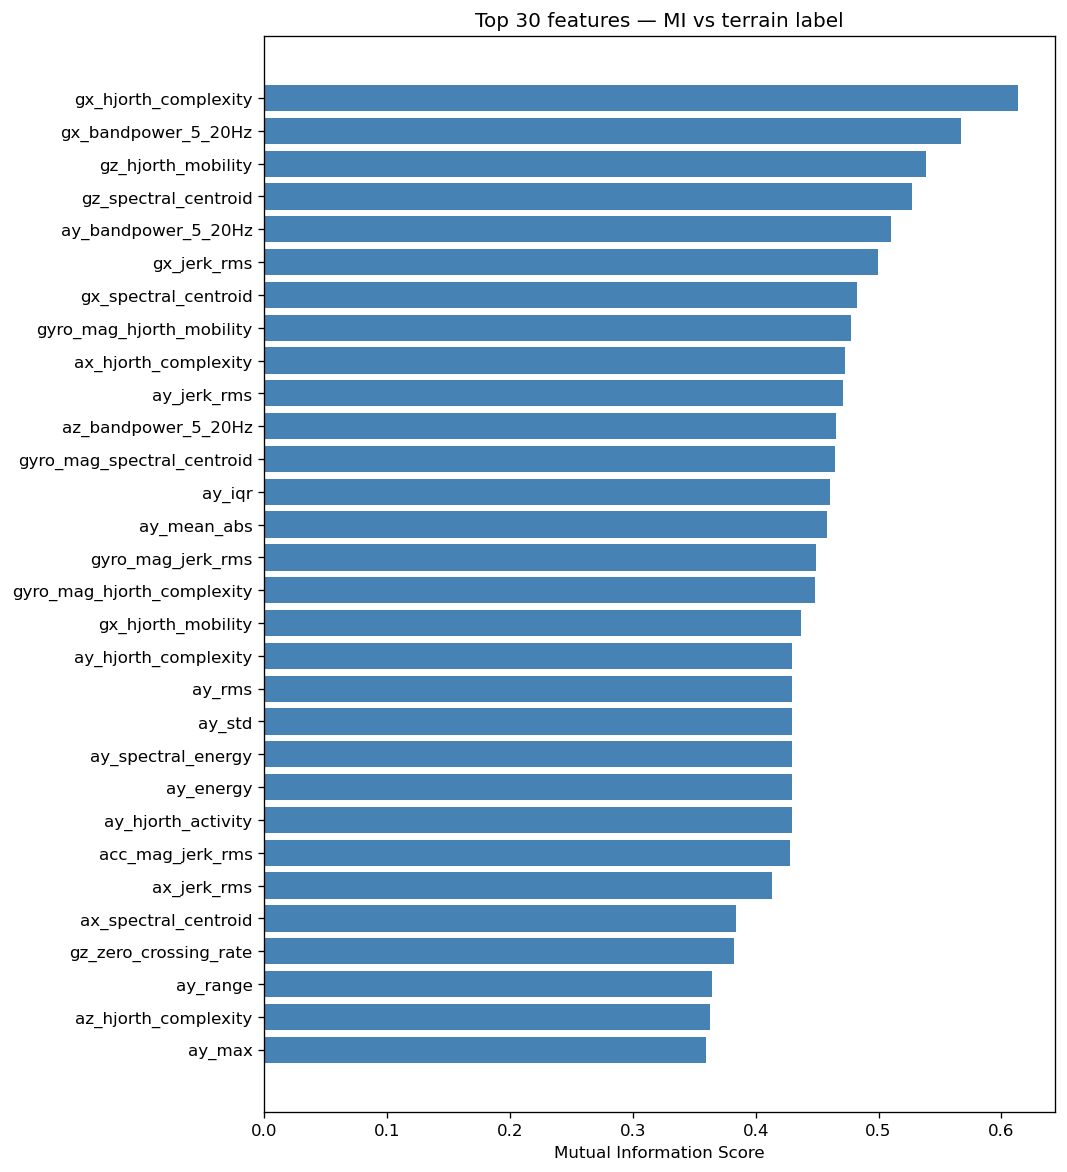
\includegraphics[width=0.85\textwidth]{Pictures/Figures/mutual_information.png}
    \caption{Top-30 features ranked by mutual information with the terrain label on the farm dataset. Gyroscope pitch and roll dynamical and frequency-band statistics, together with vertical-accelerometer band-power, dominate the leading ranks.}
    \label{fig:mi_bar}
\end{figure}

\vspace{-4mm}
\paragraph{Correlation pruning.}
The MI ranking flags relevant features but does not penalise redundancy: two highly correlated features can both rank high without either adding information beyond the other. A second pass therefore removes one feature from each pair whose absolute Pearson correlation exceeds the threshold $\rho_{\max} = 0.95$, keeping the higher-variance member:
\begin{equation}
    \mathcal{D} \;=\; \bigl\{
        j : \exists\, i \neq j \text{ with }
        |\mathrm{corr}(x_i, x_j)| > \rho_{\max}
        \text{ and } \mathrm{var}(x_j) \le \mathrm{var}(x_i)
    \bigr\}.
    \label{eq:corr_pruning}
\end{equation}
The threshold $\rho_{\max} = 0.95$ is conservative: only near-collinear pairs are removed, so the pruned table preserves all genuinely independent information. The three odometry columns are excluded from the aggressive pruning step and kept in the table for downstream diagnostics, since dropping them would make the speed-regime ablation in \Cref{sec:bg-vel} hard to perform post-hoc. The combined MI-then-correlation procedure is the standard recipe in the activity-recognition and condition-monitoring literature~\cite{Vergara2014,Bao2004} and is also applied, at a fold-local level, inside the cross-validation loop in \Cref{ch:classification}.

\begin{figure}[H]
    \centering
    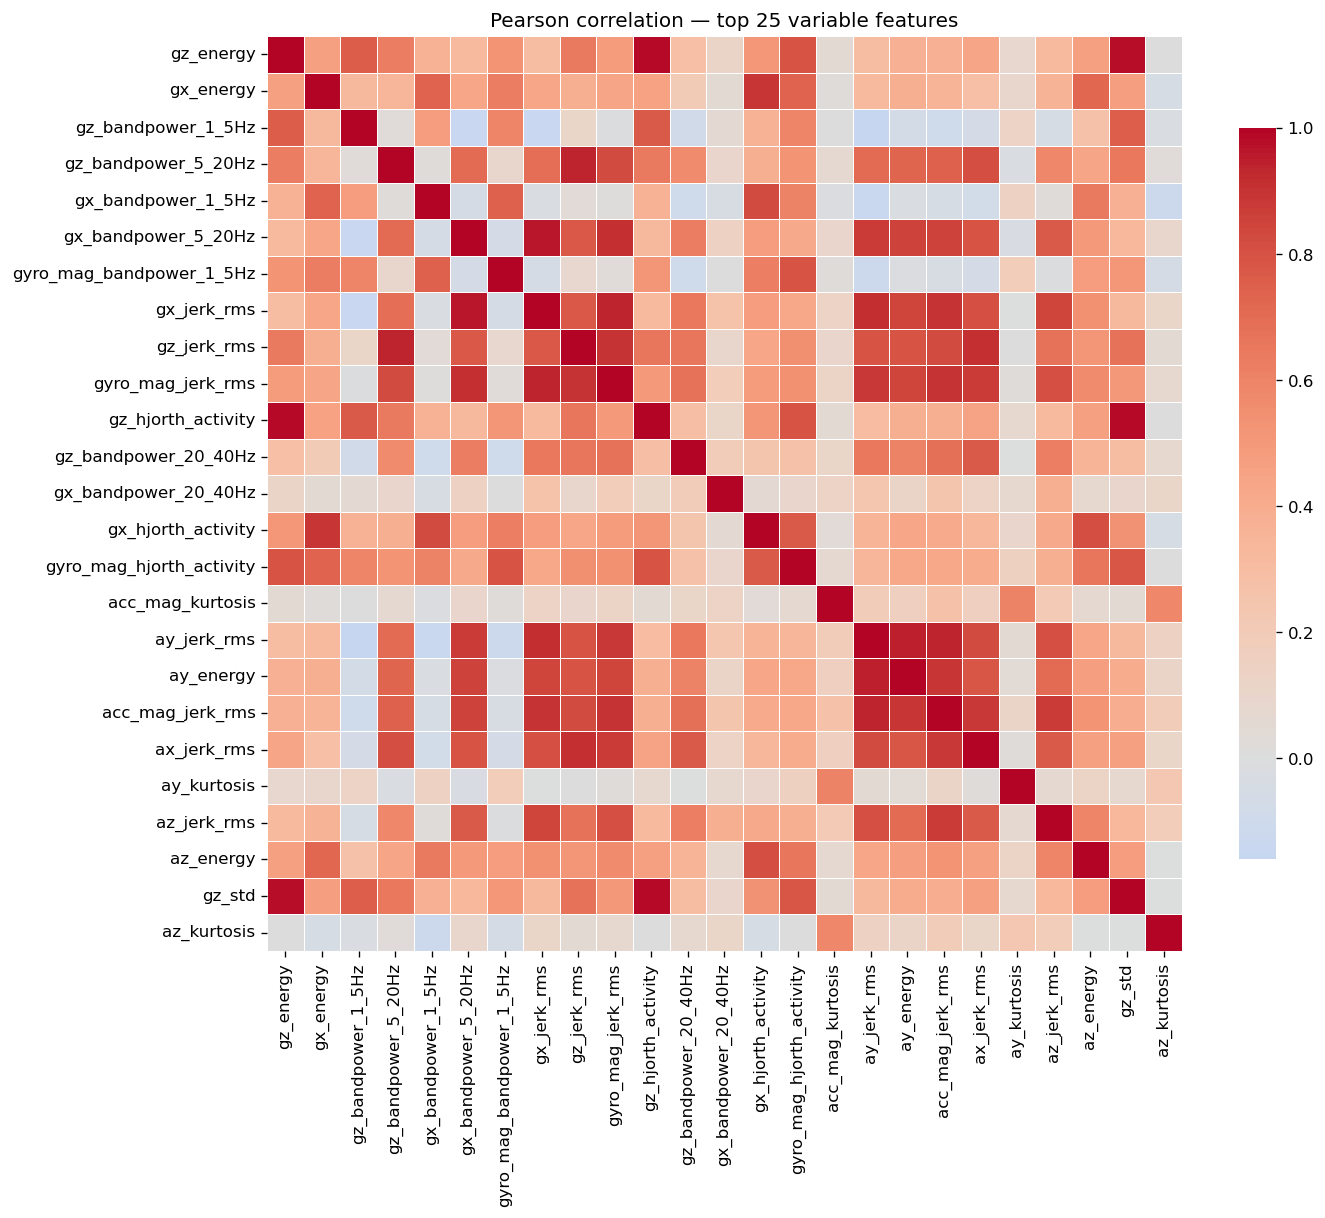
\includegraphics[width=0.80\textwidth]{Pictures/Figures/corr_heatmap.png}
    \caption{Pearson correlation heatmap of the top-25 most variable features in the farm dataset after MI ranking and correlation pruning.}
    \label{fig:corr_heatmap}
\end{figure}

\vspace{-4mm}
\subsection{Sanity Check: Low-Dimensional Embeddings}

To verify that the engineered features carry discriminative information beyond any single column, the pruned farm dataset is projected into two dimensions using principal-component analysis (PCA) and t-distributed stochastic neighbour embedding (t-SNE)~\cite{vanderMaaten2008}. Both projections are computed on the standardised feature table; t-SNE is run on a stratified subsample (capped at $2\,500$ rows) to keep the computation tractable while preserving class proportions.

\begin{figure}[H]
    \centering
    \begin{subfigure}[b]{0.48\textwidth}
        \centering
        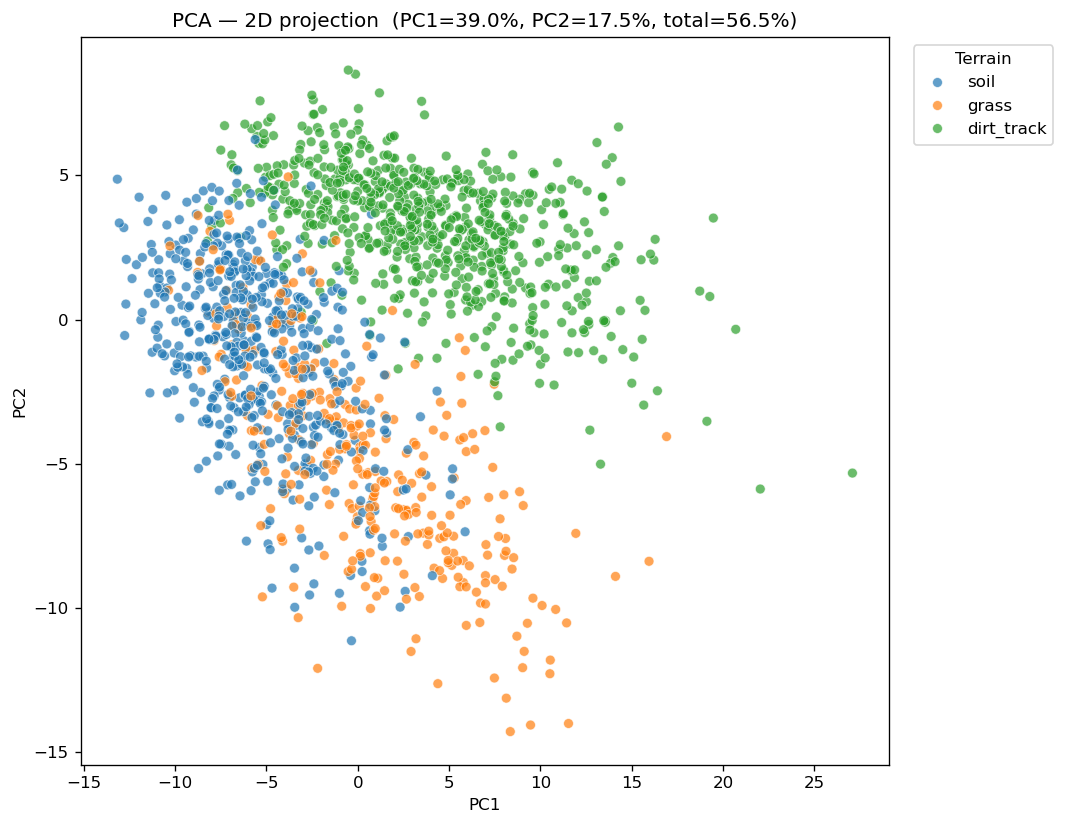
\includegraphics[width=\textwidth, height=5cm]{Pictures/Figures/pca_2d.png}
        \caption{PCA}
        \label{subfig:pca}
    \end{subfigure}
    \hfill
    \begin{subfigure}[b]{0.48\textwidth}
        \centering
        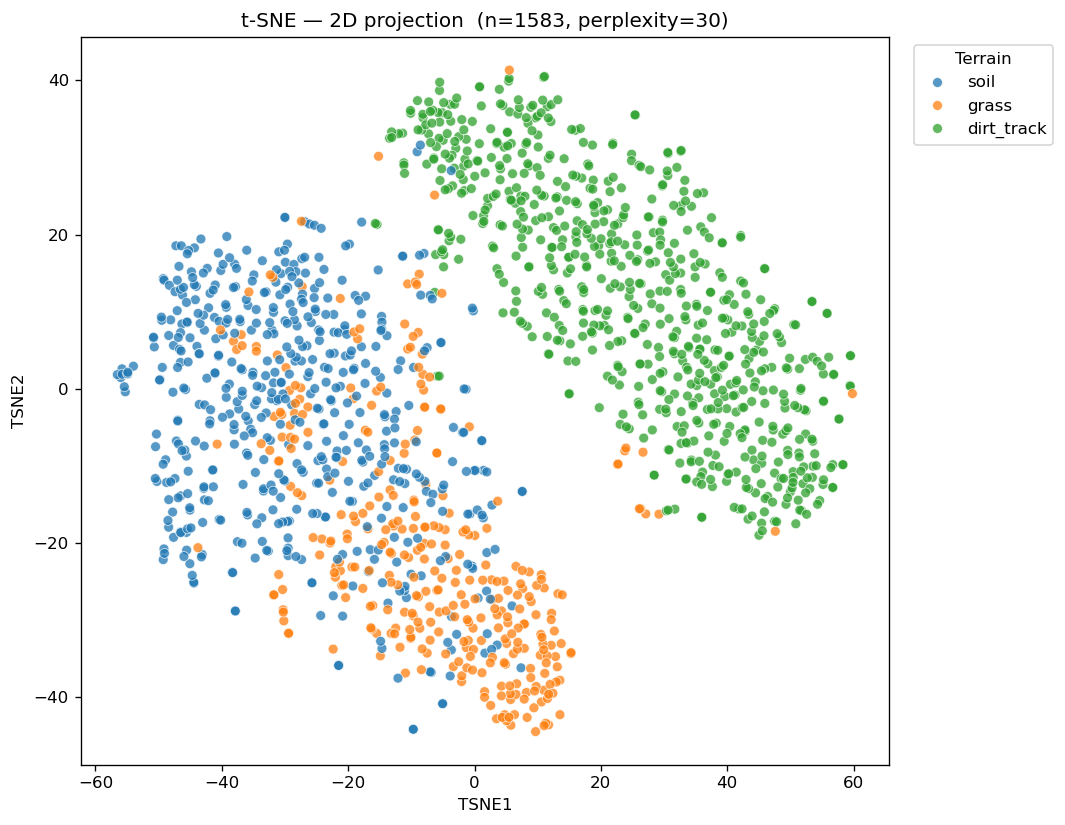
\includegraphics[width=\textwidth, height=5cm]{Pictures/Figures/tsne_2d.png}
        \caption{t-SNE}
        \label{subfig:tsne}
    \end{subfigure}
    \caption{Low-dimensional embeddings of the pruned farm feature table, coloured by terrain class. PCA (left) shows overall global structure; t-SNE (right) reveals finer class clustering.  Both projections are computed on standardised features.}
    \label{fig:embeddings}
\end{figure}

PCA captures only a small fraction of the total variance in its first two components but already separates the broad outline of the classes; t-SNE produces much tighter per-class clusters and confirms that the pruned feature table is well-separated in a non-linear sense. The detailed class-by-class separability and its implications for the choice of classifier family are taken up in \Cref{ch:results}.

\subsection{Output of the Feature Stage}

For each location, the feature-engineering pipeline writes the following artefacts under \texttt{data/processed/}:
\begin{itemize}
    \item \texttt{windowed\_features.csv} --- the full per-window feature table prior to selection.
    \item \texttt{dataset\_A\_features.csv} and \texttt{dataset\_A\_pruned.csv} --- the full-speed table and its correlation-pruned counterpart.
    \item \texttt{dataset\_B\_features.csv} and \texttt{dataset\_B\_pruned.csv} --- the low-constant-speed table and its pruned counterpart.
    \item \texttt{top\_mi\_features.json} --- the top-$N$ feature shortlist by mutual information, with a separate \texttt{top\_mi\_features\_dataset\_B\_3class.json} holding the campus 3-class merged-label shortlist.
\end{itemize}
These tables, together with the raw windowed signals stored in \texttt{raw\_windows\_cnn.parquet}, form the input to the classifier benchmark in \Cref{ch:classification}.
